\section{MSI-Based Cache Coherence Protocol}
\label{sec:System}

We have chosen as our concrete example a hierarchical MSI
protocol~\cite{MSI}. Logically, the system is organized in a tree
structure, with the root connected to the main memory and each leaf interfaced
with a processor (Figure~\ref{hier}). The system is parameterized by the shape
of the tree, and each node can have any number of children.
In the following, $\leaf(c)$ indicates
that a cache $c$ is a leaf, and $\parent(c,p)$ indicates that $p$ is the parent of
$c$.

Each node contains the fields mentioned in Figure \ref{hier}. We will
explain what the fields mean in the following discussion.

\begin{figure}
\centering
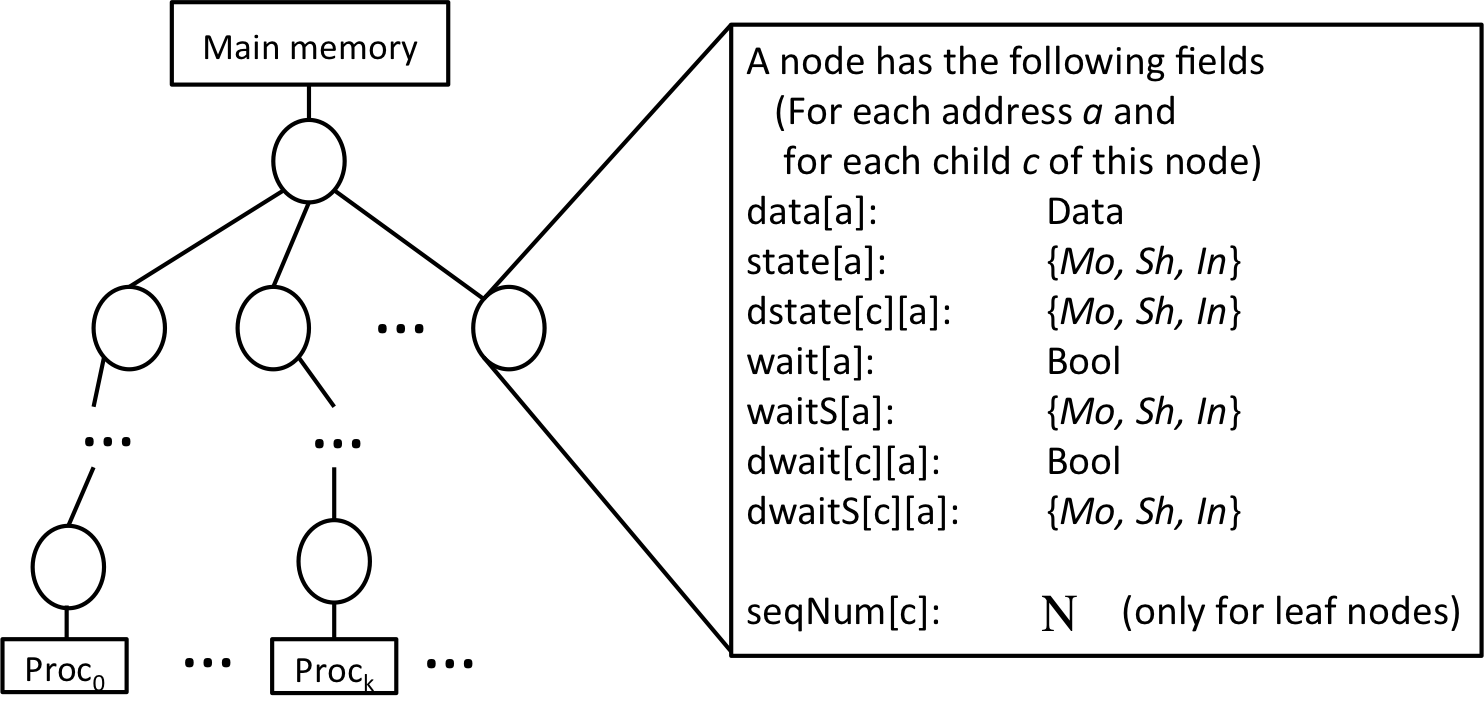
\includegraphics[scale=.5]{hier}
\caption{A cache hierarchy, and the fields in each node}
\label{hier}
\end{figure}

Input and output happen at the leaves in the form of memory requests
issued from and responses issued to the associated processors. These will be
represented by two mappings, one from $\mathbb{N}$ to requests and the other
from $\mathbb{N}$ to responses. For each leaf $c$, $c.\pos$ represents the
sequence number of the next request to process; it is set to $0$ initially.
\adamc{Add processors and main memory, labeled explicitly, to the diagram?}

Each node maintains a permission state for each address $a$, $c.\state[a]$, in
addition to the data associated with the address, $c.\data[a]$. The permission
state denotes which operations may be performed on the data. An address may be
in the \emph{read-write} state \Mo{} (for ``modifiable''),
the \emph{read-only} state \Sh{} (for ``shared''), or in the \emph{invalid} state
\In{} (indicating that it may be neither read nor written). The options form a natural
total order of permissions ($\In < \Sh < \Mo$). For a leaf cache, the meaning
of these permission states is straightforward: a load request may be processed
only if the leaf is at least in the \Sh{} state, and a store request may be
processed only if it is in the \Mo{} state. The state of a non-leaf cache indicates
an \emph{upper bound} on the permission level of any cache in the associated subtree.
If a cache does not include a particular location,
we consider that address to have permission \In.  Initially, all addresses in
each cache are in the \In{} state, save for those in the root cache (i.e., main memory),
which are in the \Mo{} state.

%Of course, all these invariants have to be enforced by the protocol.

Each non-leaf cache also keeps a (possibly stale) copy of the permission state of
each of its children in a \emph{directory} for every address. The directory
entry for a cache $c$ whose parent is $p$ for address $a$ is denoted by
$p.\dstate[c][a]$. A directory entry for a cache is never
less than the actual cache's permission state for the corresponding address.

In order for a cache to change to a higher state for a given address, \ie{}
\emph{upgrade}, it has to \emph{request} its parent.  For changing to a lower
state, \ie{} \emph{downgrade}, it has to notify its parent of the downgrade
using a \emph{response} message.  Similarly, for a parent to force a child to
downgrade for an address (in order to give permissions to a different child),
or equivalently, to downgrade the parent's directory for the child and address,
it has to \emph{request} that child to downgrade, and a parent can notify a
child about upgrading the child's state, or equivalently, about upgrading the
parent's directory state for the child, by sending a \emph{response} message.

Each cache is connected to its parent cache using 3 logical FIFO connections:
(a) \cpReq{} channel to transmit requests from the child to the parent, (b)
\cpResp{} channel to transmit responses from the child to the parent, and (c)
\pc{} channel to transmit both request and response messages from parent to
child. 

We have dedicated channels between each parent-child pair. The three channels
are indexed by the name of the child that uses that channel (denoted by
$\textit{ch}[c]$ for the \textit{ch} channel associated
with cache $c$).  Figure~\ref{format} shows the fields of the messages
transmitted in the 3 channels between caches. In each of the channels $ch$, a
message $m$ can be enqueued ($\enq(ch, m)$) or dequeued ($\deq(ch)$), and the
channels can be examined for the first element ($\first(ch)$) or for
availability of any message in the channel ($\avail(ch)$). Each of these
channels start out empty, \ie{} $\forall ch. \; \neg \avail(ch)$, initially.

\begin{figure}
\begin{subfigure}{6.8cm}
\begin{tabular}{|lp{5.8cm}|}
\hline
\multicolumn{2}{|c|}{A message in \cpReq{} channel}\\
\hline
\from: & Current state of child\\
\myto: & Desired (higher) state of child\\
\addr: & Address associated with the request\\
\hline
\hline
\multicolumn{2}{|c|}{A message in \cpResp{} channel}\\
\hline
\from: & Current state of child\\
\myto: & Downgraded state of child\\
\addr: & Address associated with the request\\
\data: & Data associated with the address, if necessary\\
\hline
\end{tabular}
\end{subfigure}
\begin{subfigure}{5.4cm}
\begin{tabular}{|lp{4.4cm}|}
\hline
\multicolumn{2}{|c|}{A message in \pc{} channel}\\
\hline
\typ: & \Req{} (for requests) and \Resp{} (for responses)\\
\myto: & Desired (lower) directory state of a child for \Req{} and upgraded
directory state of a child for \Resp{}\\
\addr: & Address associated with the request\\
\data: & Data associated with the address if necessary (for \Resp{} only)\\
\hline
\end{tabular}
\end{subfigure}
\caption{Data types for messages between caches
\adamc{Names here don't match those in the preceding text.}}
\label{format}
\end{figure}

In addition to the actual permission states, each cache also maintains a
temporary \emph{wait state} for each address to deal with transitioning between
permission levels. The wait state consists of two parts: (a) a Boolean
representing whether the cache has sent a request to its parent cache earlier
and is waiting for a response (denoted by $c.\wait[a]$ for address $a$) and (b)
one of the three values \Mo, \Sh{} or \In{} representing the state upgrade that
the cache is waiting to make (denoted by $c.\waitS[a]$ for address $a$).
Similarly, each non-leaf cache has the corresponding wait states for its
directory.  $p.\dwait[c][a]$ denotes that cache $p$ is waiting for a response
from its child $c$ for address $a$, and $p.\dwaitS[c][a]$ denotes the state to
which $p$ is waiting for $c$ to downgrade. Both \wait{} and \dwait{} are
\False{} initially for all caches and addresses,
because no cache is waiting for any response from either its child or its
parent initially.

The behavior of the system is described via the atomic state transitions, which
are effectively a nondeterministic operational semantics. These transitions
have two parts: (a) the guard dictating when the transition can fire, and (b)
the action defining how the state of the system changes when the transition
happens. Logically, these transitions happen one at a time.  Figure~\ref{trans}
gives the atomic transitions for the MSI protocol.  The actions in the
transitions in Figure \ref{trans} show only the specific states that change,
and other state components are assumed to remain the same.  The notation ($x
\Leftarrow y$;) in a transition indicates setting of a specific state $x$ of
the overall system to value $y$.

We first give an intuition on how the transitions work in the common case.
A cache can decide, spontaneously, to upgrade its state,
in which case it sends an upgrade request to its parent. The parent then makes
a local decision on whether to send a response to the requesting child or not
(based on its directory approximation, and its own state). If its own state is
lower the requested upgrade, then it cannot handle the request. The parent
must instead decide to upgrade its state -- the transition for doing so has
nothing to do with the incoming request.  Once the parent's state is not lower
than the requested upgrade, it makes sure that the rest of its children are
``compatible'' with the requested upgrade. If not, the parent must send
requests to the incompatible children to downgrade -- again the transition for
doing so has nothing to do with the incoming request. If the children are
compatible and its own state is higher, then the request can be handled and a
response is sent. Each of the transitions is explained in greater detail below.

Figure~\ref{childside} shows the transitions that result in an upgrade of the
state of a cache. It involves a cache sending an upgrade request to the its
parent if the cache is not already waiting for some response for that address
from the parent (ChildSendReq). This request is received by the parent
(ParentRecvReq). If the directory entries for all of the other children are
\emph{compatible} with the upgrade request, and the parent's permission state has
at least the requested value, it sends an upgrade response to the cache, while
changing the appropriate directory state. The notation \compat{} used in
the ParentRecvReq transition of Figure \ref{trans} is defined as follows:
\begin{multline*}
\small
\compat(p, c, a, s) = \forall i \ne c. \;
\mylet s_i := p.\dstate[i][a] \myin\\
 (s = \Mo @-> s_i = \In) \wedge (s = \Sh @-> s_i = \Sh) \wedge (s = \In @-> s_i = \Mo)
\end{multline*}
Finally, the child cache receives the response from the parent (ChildRecvResp)
and sets its state while resetting its wait state if the response contains the
desired upgrade.

Figure~\ref{parentside} shows the similar sequence of transitions that results
in downgrading a cache's directory entry for one of its children $c$. The
difference is in the guard for the ChildRecvReq transition: the directory entry for
each of $c$'s children should not be greater than the requested
downgrade, in order for $c$ to accept a request and send a downgrade
response.

Figure~\ref{childextra} shows transitions that happen in a non-root cache due
to the presence of \emph{voluntary} responses, which model eviction of a
location from a cache to make room for a new location. This eviction usually
causes the permission state of the cache for that address to go to $\In$, while
we allow any downgrade to take place voluntarily.  We use the same \cpResp{}
FIFO for such a message. Such a voluntary response for an address can take
place only if the cache is not waiting for a response from its parent for that
address (ChildVolResp).

Because of the presence of voluntary responses, a child could have already
downgraded to a state required by a downgrade request from its parent. In such
a case, the child simply drops the downgrade request (ChildDropReq).

Figure~\ref{procside} shows the transitions that serve a processor's request in
the leaf caches. LoadReq and StoreReq show the processing of a load and store
request, respectively. In the case of a store request, the data in the cache
for the requested address is updated with that supplied in the request. We do
not explicitly show the response generated by the cache in case of a load
request; in a real system, the data in the cache for the requested address is
sent back to the processor. When a LoadReq or StoreReq happens at a cache $c$
pertaining to address $a$, the \Response{}, needed in the definition of store
atomicity, is generated as follows: the \labelR{} field contains a pair $(c, c.\pos)$,
the \dataR{} field contains the value $c.\data[a]$, and the \timeR{} field
contains the number of transitions that have happened in the system before
the current transition, intuitively denoting the time at which this transition
takes place.


\begin{figure}
\small
\centering
\begin{subfigure}{\textwidth}
\centering
\begin{tabular}{|ll|}
\hline
\multicolumn{2}{|l|}{\textbf{ChildSendReq}$(c, x, a)$: Child $c$ sending request to upgrade to $x$ for address $a$}\\
\hline
Guard: & $c.\state[a] < x \wedge c.\wait[a] = \False$\\
\hline
Action: & $c.\waitS[a] \Leftarrow x$; $c.wait[a] \Leftarrow \True$; $\enq(\cpReq[c], \langle c.\state[a], x, a \rangle)$;\\
\hline
\hline
\multicolumn{2}{|l|}{\textbf{ParentRecvReq}$(p, c)$: Parent $p$ receiving a request from child $c$}\\
\hline
Guard: & 
$\parent(c,p) \wedge \avail(\cpReq[c]) \wedge \mylet q := \first(\cpReq[c]) \myin$\\
& $p.\dwait[c][q.\addr] = \False \wedge p.\dstate[c][q.\addr] \le q.\from \wedge$\\
& $\compat(p, c, q.\addr, q.\myto) \wedge q.\myto \le p.\dstate[q.\addr]$\\
\hline
Action: & $\enq(\pc[c], \langle \Resp, q.\myto, q.\addr, $\\
& $\;\;\;%
\myif p.\dstate[c][q.\addr] = \In \mythen p.\data[q.\addr] \myelse \_\rangle)$;\\
& $p.\dstate[c][q.\addr] \Leftarrow q.\myto$; $\deq(\cpReq[c])$;\\
\hline
\hline
\multicolumn{2}{|l|}{\textbf{ChildRecvResp}$(c)$: Child $c$ receiving a response}\\
\hline
Guard: & 
$\avail(\pc[c]) \wedge \mylet r := \first(\pc[c]) \myin r.\typ = \Resp$\\
\hline
Action: & $\myif c.\state[r.\addr] = \In \mythen c.\data[a] \Leftarrow r.\data$;\\
&$\myif c.\waitS[r.\addr] \le r.\myto \mythen c.\wait[a] \Leftarrow \False $;\\
& $c.\state[r.\addr] \Leftarrow r.\myto$; $\deq(\pc[c])$;\\
\hline
\end{tabular}
\caption{Child sending upgrade request and getting back the response}
\label{childside}
\end{subfigure}

\begin{subfigure}{\textwidth}
\centering
\begin{tabular}{|ll|}
\hline
\multicolumn{2}{|l|}{\textbf{ParentSendReq}$(p, c, x, a)$: Parent $p$ sending request to child $c$ to downgrade to $x$ for address $a$}\\
\hline
Guard: & $\parent(c,p) \wedge p.\dstate[c][a] > x \wedge p.\dwait[c][a] = \False$\\
\hline
Action: & $p.\dwaitS[c][a] \Leftarrow x$; $p.\dwait[c][a] \Leftarrow \True$; $\enq(\pc[c], \langle \Req, x, a, \_ \rangle)$;\\
\hline
\hline
\multicolumn{2}{|p{\textwidth}|}{\textbf{ChildRecvReq}$(c)$: Child $c$ receiving a request from its parent and has to downgrade}\\
\hline
Guard: & 
$\avail(\pc[c]) \wedge \mylet q := \first(\pc[c]) \myin q.\typ = \Req \wedge$ \\
& $(\forall i, \parent(i, c) \rightarrow c.\dstate[i][q.\addr] \le q.\myto) \wedge q.\myto < c.\state[q.\addr]$\\
\hline
Action: & $\enq(\cpResp[c], \langle c.\state[q.\addr], q.\myto, q.\addr,$\\
& $\;\;\;%
\myif c.\state[q.\addr] = \Mo \mythen c.\data[q.\addr] \myelse \_\rangle)$;\\
& $c.\state[q.\addr] \Leftarrow q.\myto$; $\deq(\pc[c])$;\\
\hline
\hline
\multicolumn{2}{|l|}{\textbf{ParentRecvResp}$(p, c)$: Parent $p$ receiving a response from child $c$}\\
\hline
Guard: & 
$\parent(c,p) \wedge \avail(\cpResp[c]) \wedge \mylet r := \first(\cpResp[c]) \myin$\\
& $r.\from = p.\dstate[c][r.\addr]$\\
\hline
Action: & $\myif p.\dstate[c][r.\addr] = \Mo \mythen p.\data[r.\addr] \Leftarrow r.\data$;\\
&$\myif p.\dwaitS[c][r.\addr] \ge r.\myto \mythen p.\dwait[c][r.\addr] \Leftarrow \False $;\\
& $p.\dstate[c][r.\addr] \Leftarrow r.\myto$; $\deq(\cpResp[c])$;\\
\hline
\end{tabular}
\caption{Parent sending downgrade request and getting back the response}
\label{parentside}
\end{subfigure}

\begin{subfigure}{\textwidth}
\centering
\begin{tabular}{|ll|}
\hline
\multicolumn{2}{|p{\textwidth}|}{\textbf{ChildVolResp}$(c, x, a)$: Child $c$
sending a response to downgrade to $x$ for address $a$ without any request from
its parent}\\
\hline
Guard: & $(\forall i, \parent(i, c) \rightarrow c.\dstate[i][a] \le x) \wedge x < c.\state[a] \wedge c.\wait[a] = \False$\\
\hline
Action: & $\enq(\cpResp[c], \langle c.\state[a], x, a,%$\\
%& $\;\;\;%
\myif c.\state[a] = \Mo \mythen c.\data[a] \myelse \_\rangle)$;\\
& $c.\state[a] \Leftarrow x$;\\
\hline
\hline
\multicolumn{2}{|p{\textwidth}|}{\textbf{ChildDropReq}$(c)$: Child $c$
receiving a request from its parent and has already downgraded}\\
\hline
Guard: & 
$\avail(\pc[c]) \wedge \mylet q := \first(\pc[c]) \myin q.\typ = \Req \wedge q.\myto \ge c.\state[q.\addr]$\\
\hline
Action: & $\deq(\pc[c])$;\\
\hline
\end{tabular}
\caption{Other transitions at a non-root cache}
\label{childextra}
\end{subfigure}

\begin{subfigure}{\textwidth}
\centering
\begin{tabular}{|ll|}
\hline
\multicolumn{2}{|l|}{\textbf{LoadReq}$(c)$: Handling a processor's load request at a leaf cache}\\
\hline
Guard: & $\leaf(c) \wedge \mylet q := \reqFn(c, c.\pos) \myin q.\desc = \Ld \wedge c.\state[q.\addrQ] \ge \Sh$\\
\hline
Action:& $c.\pos \Leftarrow c.\pos + 1$;\\
\hline
\hline
\multicolumn{2}{|l|}{\textbf{StoreReq}$(c)$: Handling a processor's store request at a leaf cache}\\
\hline
Guard: & $\leaf(c) \wedge \mylet q := \reqFn(c, c.\pos) \myin q.\desc = \St \wedge c.\state[q.\addrQ] = \Mo$\\
\hline
\hline
Action:& $c.\pos \Leftarrow c.\pos + 1$; $c.\data[q.\addrQ] \Leftarrow q.\dataQ$;\\
\hline
\end{tabular}
\caption{Handling requests from the processor}
\label{procside}
\end{subfigure}
\caption{Atomic transitions for a cache-coherent memory subsystem}
\label{trans}
\end{figure}

Note that the atomic transitions in Figure~\ref{trans} access only local states,
\ie{} a transition can read or write states only corresponding to a single cache
and/or the channel the cache is connected to. This restriction allows such a
system to be implemented directly into hardware. Bluespec System Verilog (BSV),
for instance, directly converts these transitions into efficient synchronous
hardware. Though these transitions logically happen one by one, BSV executes
several transitions simultaneously, as long as they do not access the same
state, \ie{} do not \emph{conflict}~\cite{Hoe:TCAD,HoeArvind:TRSSynthesis1}.
Sometimes, these transitions (both the guards and the actions) may not be
amenable to single-cycle implementations in hardware. For example, writing a
register array can actually take several hardware clock cycles, though
logically it is a single transition. Karczmarek \etal~\cite{Karczmarek} have
provided a scheme to convert atomic transitions into synchronous hardware in
which each transition can span several clock cycles.
